\documentclass[a4paper]{article}

\usepackage[english]{babel}
\usepackage[utf8]{inputenc}
\usepackage{amsmath}
\usepackage{graphicx}
\usepackage{setspace}
\renewcommand{\baselinestretch}{1.5} 
\usepackage[colorinlistoftodos]{todonotes}
\usepackage{url}
\title{Gaussian processes applied to the study of chemotactic movements of droplets}

\author{Carlotta Porcelli, qbp693}

\date{\today}

\begin{document}
\maketitle

\begin{abstract}
The research hereby presented investigates the use of a Gaussian Process regression model on a dataset collected from experiments lead in the context of Artificial Chemical Life for the EVOBLISS project \cite{evobliss} at the REAL laboratory in the IT University of Copenhagen \cite{itu_real} . The experiments performed examine the chemotactic behavior of 1-Decanol droplets placed in Decanoate solutions with different pHs and molarities when a chemical gradient is introduced in the external aqueous environment. The Gaussian process model has been fit to the data collected in order to look for a combination of pH and molarity values of the decanoate solution that would allow the droplet to increase the efficiency of its chemotactic movement. 
\end{abstract}

\section{Introduction}
The movement of non-living objects in aqueous environments has been used to reproduce the chemotaxis process of a living cell, movement in a particular direction. \cite{ikea} 
\\The development of chemical systems that mimic the behavior of living systems can be useful in studying related processes in natural living systems.
\\The data exploited in this research have been collected with the usage of EvoBot \cite{evobot}, a liquid handling robot built in the context of the EVOBLISS \cite{evobliss} project. One of the goal of this project is to develop a robotic platform, which by using artificial evolution, can optimize the performance of a physicochemical system and its environment.
\\The experiments are composed of two parts, one is fixed and the other one is variable. The droplet composition and volume along with the salt gradient created, form the fixed part: their values are in fact the same in all the experiments. On the other hand, the variable part is the water phase, generated by two continuous variables: the molarity and the pH of the decanoate (Decanoic Acid) solutions. The experiments carried out by EvoBot \cite{evobot} span in continuous ranges of molarity, from 5mM to 20mM and pH from 7.0 to 12.3 to create the aqueous environment.
\\The aqueous combinations explored were created by mixing decanoate solutions at different pHs and adding water to get the molarity desired. Once the solutions were ready, a 1-Decanol droplet was added to the system and a salt gradient was created adding a solution of NaCl.
The salt gradient allows the droplet to move from the point in which it was inserted into the system to the salt source, following the gradient created by the salt.
In each experiment the droplet movement is tracked for a total time of 60 seconds. The implementation of the tracking assigns a \textit{fitness value} based on the speed and the spatial precision of the droplet. High values represent good chemotactic movements.
\\ Figure \ref{fig:droplet_screen} shows an example of the tracking of one individual. The tracking starts at the initial position where the droplet is placed. The blue path is composed of the centroids of the droplet after its movement. 
\newpage
The ‘END’ point is where the program stopped tracking the droplet because it reached the proximities where the salt was added, \textit{salt source}. The droplet reached efficiently the salt source and the fitness value registered is 0.120086. 

\begin{figure}
	\centering
	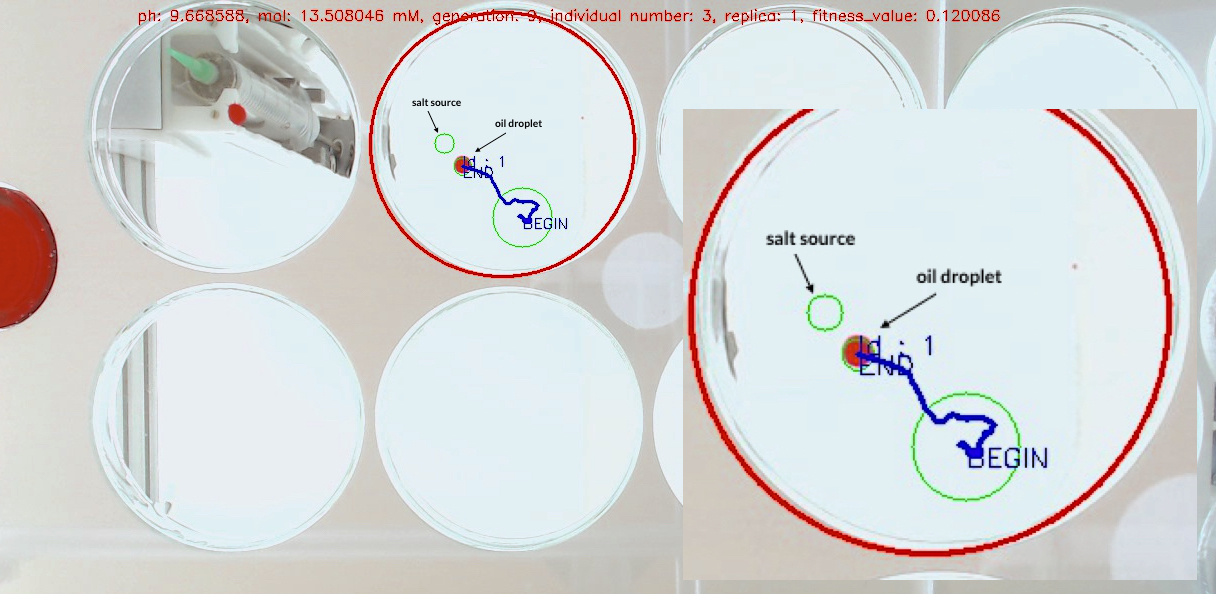
\includegraphics[width=1\textwidth]{droplet_screen2.jpg}
	\caption{Example of the tracking of an individual. This image is saved for all the experiments and contains the information about the individual, including the pH and molarity of the solution tested, in this case pH=9.66 and molarity=13.50.}
	\label{fig:droplet_screen}
\end{figure}

The aim of the project hereby presented is to make an estimation on the values of pH and molarity forming a decanoate solution in which the droplet performs a smooth and precise chemotactic movement. In this mean, a Gaussian regression model is used to characterize a non-linear relationship between the two variables (pH and molarity).
In a classic linear regression algorithm, it is assumed that a dependent variable y can be modeled as a function of one or more independent variables X in the form of $y=f(x)+\epsilon$.
The choice of the GP approach relies on the facts that it finds a distribution over the possible functions \textit{f(x)} consistent with the observed data. Moreover, the observations occur in a continuous domain. 
\newpage
\section{Materials and methods}

\subsection{The dataset}
The data set used is composed of 73 experiments. As shown in Table \ref{table} the first two columns contain the values of pH and molarity of the solutions tested, the last column specifies the fitness values computed after the tracking of the droplet. 
To obtain the data here studied, an evolutionary algorithm has been performed on the chemical system to optimize the ph and molarity of the aqueous solutions for the chemotactic movement. 

\begin{table}[]
	\centering
	\caption{First 4 data points}
	\label{table}
	\begin{tabular}{|c|c|c|}
		\hline
		\textbf{pH} & \textbf{molarity} & \textbf{fitness values} \\ \hline
		10.07 & 11.35   & -0.027            \\ \hline
		10.94 & 10.03      & -0.017            \\ \hline
		9.72  & 8.97     & -0.032            \\ \hline
		9.84 & 12.44       & 0.105             \\ \hline
	\end{tabular}
\end{table}

\subsection{Software used}
The library from which the Gaussian process regression model has been implemented is the GPy framework from the Sheffield machine learning group. \cite{gpy}

\subsection{The Gaussian Processes}
The task of building regression models to characterize non-linear relationships between variables often involves extensive model selection procedures to ensure that the most appropriate model is chosen.
An alternative is to use a Bayesian strategy to model the unknown underlying function.
Modeling data using Gaussian distributions in some cases would not seem to be any gain because of the reduced flexibility that those distributions have. 
A Gaussian process is defined as probability distribution over functions f(x) so that the set of values of f(x) evaluated on a set of points ${ x }_{ 1 },...,{ x }_{ N }$ jointly have a Gaussian distribution.
\\A Gaussian process (GP) assumes that a $p(f({ x }_{ 1 }),...,f({ x }_{ N }))$ is jointly Gaussian with some mean $\mu(x)$ and covariance $ \sum { (x) } $ given by $\sum _{ ij }^{  }{ =k({ x }_{ i },{ x }_{ j }) } $, where k is a positive definite kernel function \cite{gp_process}.
The covariance represents a form of distance or similarity. Considering two input points ${x}_{i}$ and ${x}_{j}$ with corresponding observed values ${y}_{i}$ and ${y}_{j}$, if the inputs are close to each other, it is expected that that ${y}_{i}$ and ${y}_{j}$ will be close as well. This measure of similarity is embedded in the covariance function.
Since the key assumption in GP modeling is that the data can be represented as a sample from a multivariate Gaussian distribution, we have that
\begin{equation}
\begin{bmatrix} y \\ { y }_{ * } \end{bmatrix}\sim N \left( 0,\begin{bmatrix} K & { K }^{ T } \\ { K }_{ * } & { K }_{ ** } \end{bmatrix} \right)
\end{equation}
Where y is the observed value, ${y}_{*}$ is the prediction and K is the covariance matrix. The interest is on the conditional probability $p({y}_{*}|y)$ that follows a Gaussian distribution:
\begin{equation}
{ y }_{ * }|y\sim N({ K }_{ * }{ K }^{ -1 }y,{ K }_{ ** }-{ K }_{ * }{ K }^{ -1 }{ K }_{ * }^{ T })
\end{equation}

\subsubsection{Choice of Kernel}
The kernel used to describe the covariance function expected in the dataset is the Radial-basis function (RBF) kernel defined on two samples x and x' as: 
\begin{equation}
	K({ x },{ x' })=\sigma ^{ 2 }exp\left( -{ \frac { \| { x }-{ x' }\| ^{ 2 } }{ 2l ^{ 2 } }  } \right)
\end{equation}
Where $\| { x }-{ x' }\| ^{ 2 }$ is the squared Euclidean distance between the two samples and $l$ is the length-scale free parameter describing how smooth the function has to be and $\sigma ^{ 2 }$ the variance. 
The kernel used in the GP model has been implemented as follows:
{\setstretch{1}
	\\\textit{kg = GPy.kern.RBF(input\_dim=2, variance=0.5, lengthscale=1., ARD=True)}
}
Where the \textbf{input\_dim} parameter represents the dimension of the input space, equals to two variables; the \textbf{variance}, determining the variation of function values from their mean, has been set to 0.5 and the \textbf{lengthscale} to 1. The flag \textbf{ARD=True} indicates having one lengthscale parameter per dimension.

\subsubsection{Model parameters and optimization}
The model has been implemented using the kernel in the above section and the noise variance parameter set to 1. This parameter specifies how much noise is expected to be present in the data.
{\setstretch{1}
\\\textit{model = GPy.models.GPRegression(XTrain, y\_train\_set\_, kernel=kg, normalizer=False, noise\_var=1.)}
}
\\The model has been later fit to the data using the 
\textbf{model.optimize()} function with maximum number of function evaluations equals to 1000. 
A value of 10 has been specified for the parameter \textbf{n\_restarts\_optimizer}, which rusn the optimization algorithm as many times as specified, using randomly-chosen starting coordinates to avoid finding a local, rather than a global, maximum in the marginal likelihood.

\section{Results}
The plot in Figure \ref{fig:distributuion_data_set} shows the distribution over the experimental space of the data set. The points are colored accordingly to their fitness value.
The plot in Figure \ref{fig:before_fit_non_norm} shows the Gaussian density distribution of the data before fitting the model. 
\\The plot in Figure \ref{fig:after_fit_non_norm} shows the Gaussian density distribution after fitting the model on the data set. 

\begin{figure}
	\centering
	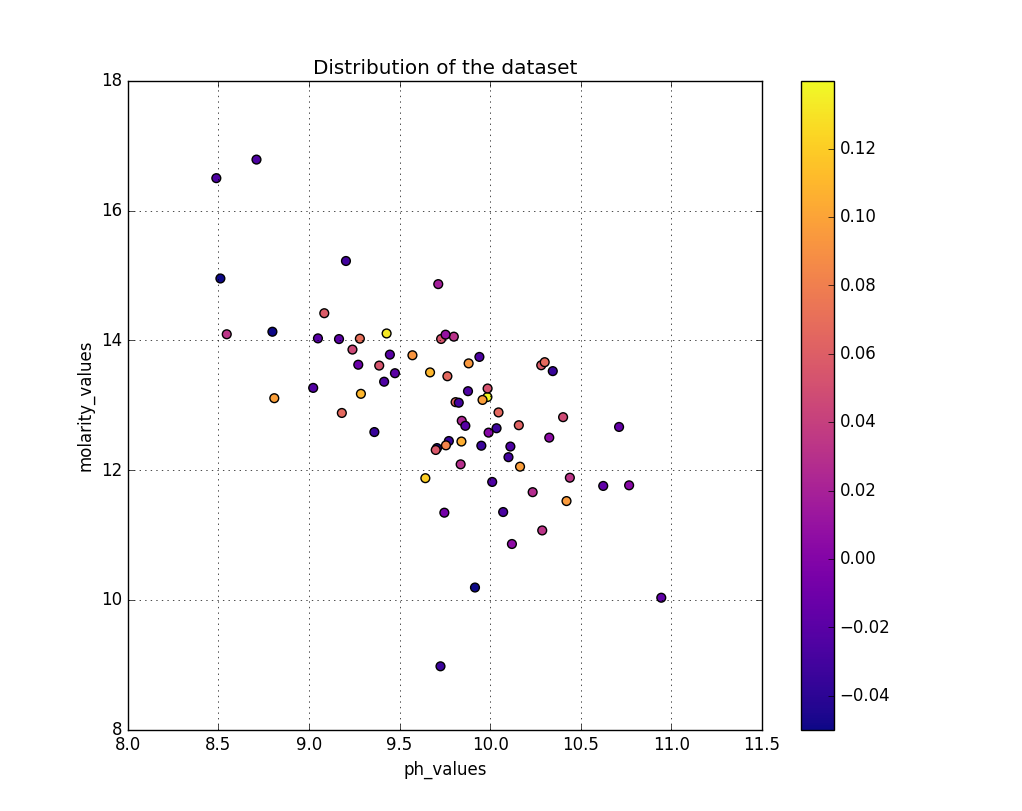
\includegraphics[width=1\textwidth]{train_data_set_scatter.png}
	\caption{Distribution of the data set colored by fitness values}
	\label{fig:distributuion_data_set}
\end{figure}

\begin{figure}
\centering
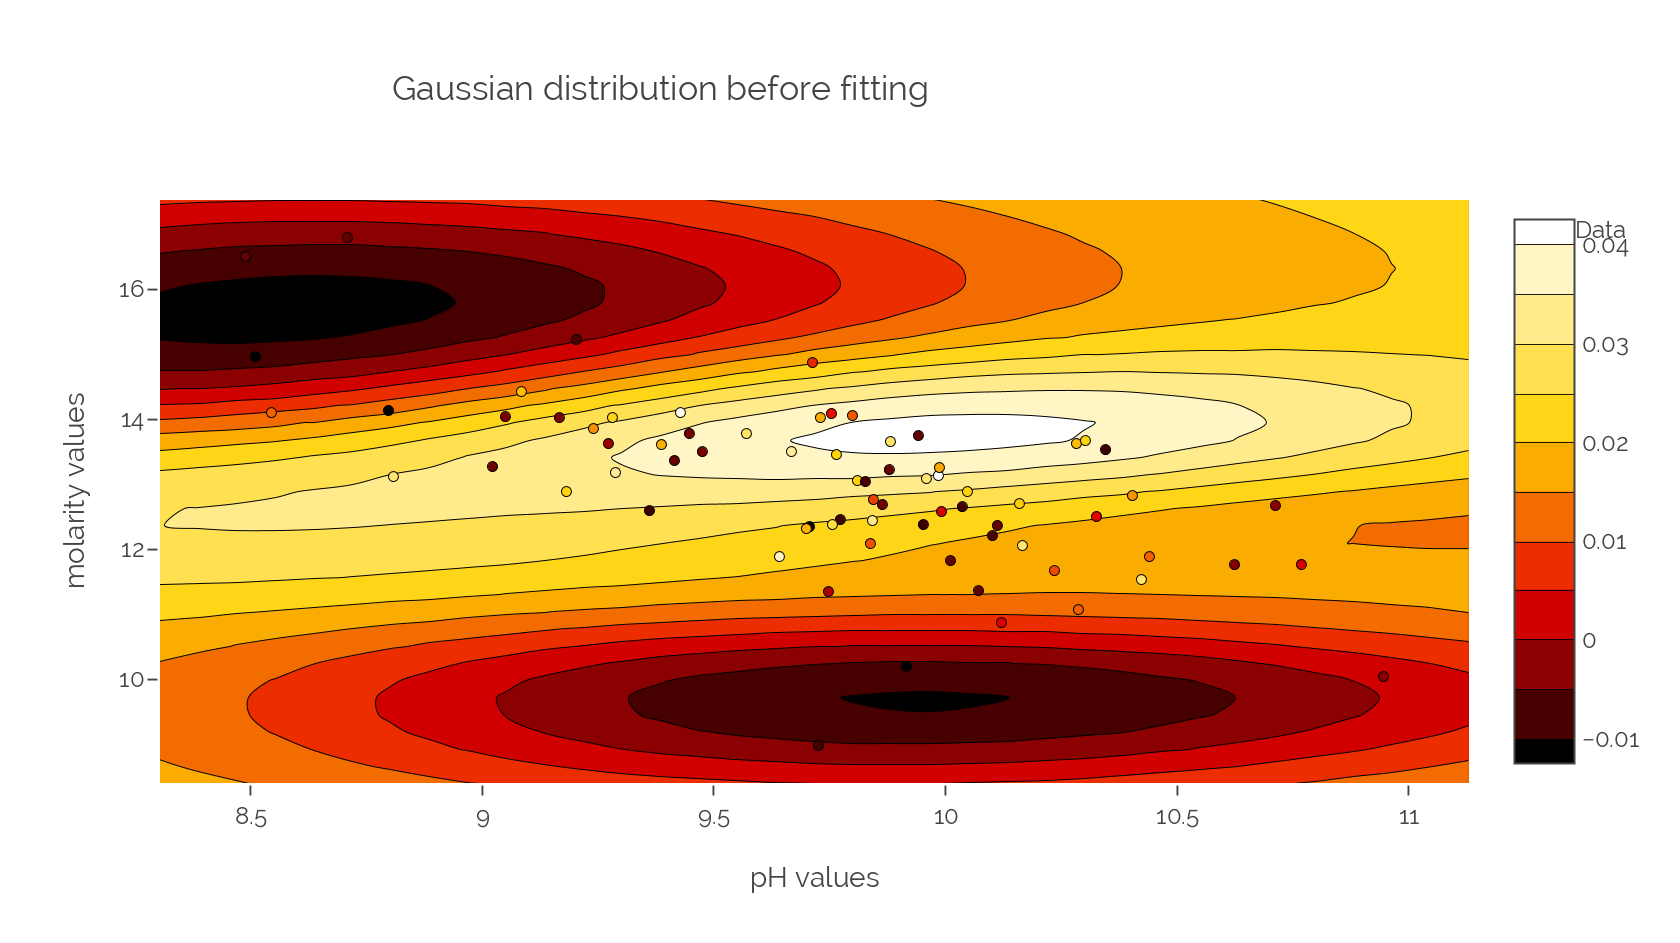
\includegraphics[width=1\textwidth]{before_fit_non_norm.png}
\caption{Gaussian distribution before fitting the  non normalized data}
\label{fig:before_fit_non_norm}
\end{figure}

\begin{figure}
	\centering
	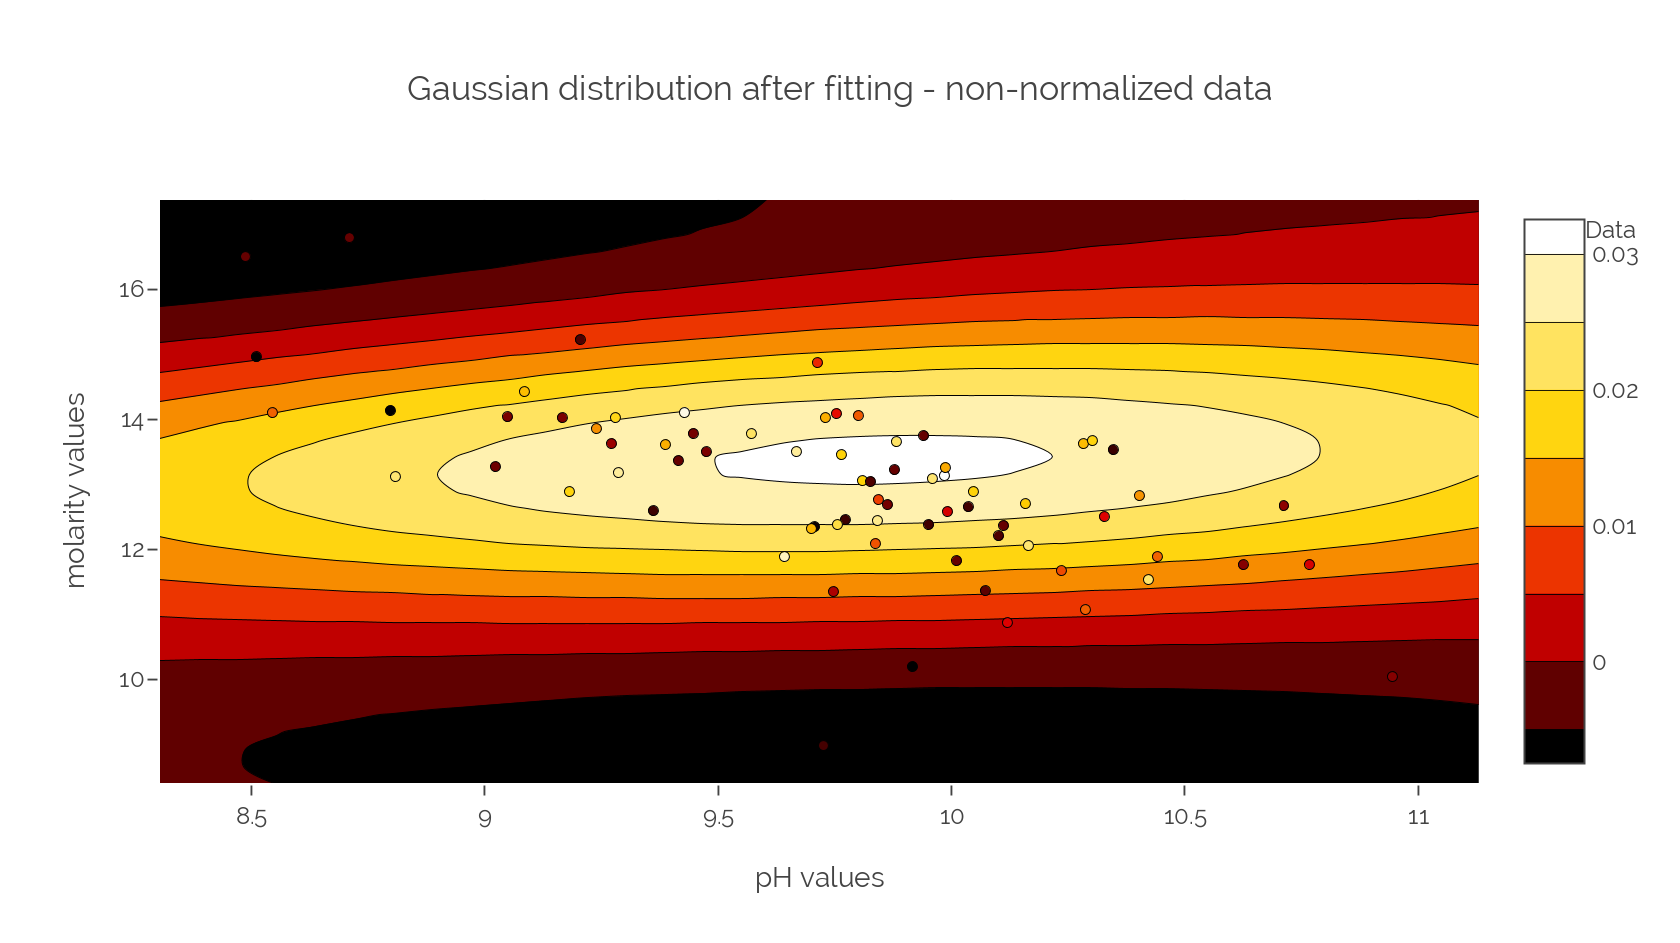
\includegraphics[width=1\textwidth]{after_fit_non_norm.png}
	\caption{Gaussian distribution after fitting the  non normalized data}
	\label{fig:after_fit_non_norm}
\end{figure}
\newpage
\section{Discussion}
From the plot in Figure \ref{fig:after_fit_non_norm} it is possible to observe the lighter area bounded by values $9.5<pH<10.2$ and $12<molarity<14$. In this area the samples should get higher fitness values than the darker areas depicted around it. However, it can be observed that many samples in that area have darker color, meaning lower fitness values. This could be explained by the fact that a high number of tested individuals, even having very similar pH and molarity values, produced very different results. 
This is also shown in the plot in Figure \ref{fig:distributuion_data_set} where many points close to each other, or almost overlapping, have different fitness values. It has to be said that, being the data a result of evolutionary experiments, some areas of the search space are oversampled, this is where the evolutionary algorithm converged.
The chemical system studied is unfortunately highly unstable. In many cases it has been noticed that Marangoni flows, superficial tensions between droplets and the edge of the Petri dish or air flows, affected the movements of the droplet resulting in low fitness values even though the same aqueous phase might have produced higher results in the previous experiment. 
A collection of data from previous experiments, not presented here, showed that a high level of noise was present. To smooth the noise in the system the number of experiments for each individual was increased to four and the final fitness value of each experiment was chosen to be the median of the four replicas instead of the average, in order to minimize the influence of the outliers. Regrettably it seems that there still is a high level of noise in the evaluation.
 
\subsection{Future work}
To solve the problems related to the chemical system, future work has been programmed to improve the results of these experiments. A change in the protocol for making the solutions is being studied and a covering to avoid air flows from the outside has been designed. 
On the computational side, different type of kernels or combinations of them could be explored to check for different results. 
Even though the system is noisy, experiments within the above found range of pH and molarity could be lead in order to check if the fitness values match the ones indicated from the model. 

\newpage

\begin{thebibliography}{9}
	
\bibitem{evobliss}
	\url{https://blogit.itu.dk/evoblissproject/overview/progress/artificial-chemical-life/}, August 19, 2017.
	
\bibitem{itu_real}
	\url{https://real.itu.dk/projects/evobliss/}, August 19, 2017.

\bibitem{ikea}
	J. Cejkova, M. Novák, F. Stěpánek and M.M. Hanczyc (2014) Dynamics of tactic droplets in salt concentration gradients. \textit{Langmuir} 30(40): 11937-44.

\bibitem{evobot}
		Andres Faina, Farzad Nejatimoharrami, Kasper Støy, Pavlina Theodosiou, Benjamin Taylor, Ioannis Ieropoulos. "EvoBot: An Open-Source, Modular Liquid Handling Robot for Nurturing Microbial Fuel Cells" in  \textit{Proceedings of the Artificial Life Conference 2016} .United States: MIT Press, 2016, pp. 626--633.

\bibitem{gpy}
	GPy: A Gaussian process framework in python -
	\url{http://github.com/SheffieldML/GPy}, August 19, 2017.

\bibitem{gp_process}
Robert, Christian. "Machine Learning, a Probabilistic Perspective." (2014): 62-63.


\end{thebibliography}
\end{document}